\chapter{System Schematics and Architecture}

\section{Global Metabiotic Architecture}
The HAWRA system is a multi-layered cyber-physical architecture where the biological substrate is controlled by a high-level logic layer.

\begin{figure}[h!]
\centering
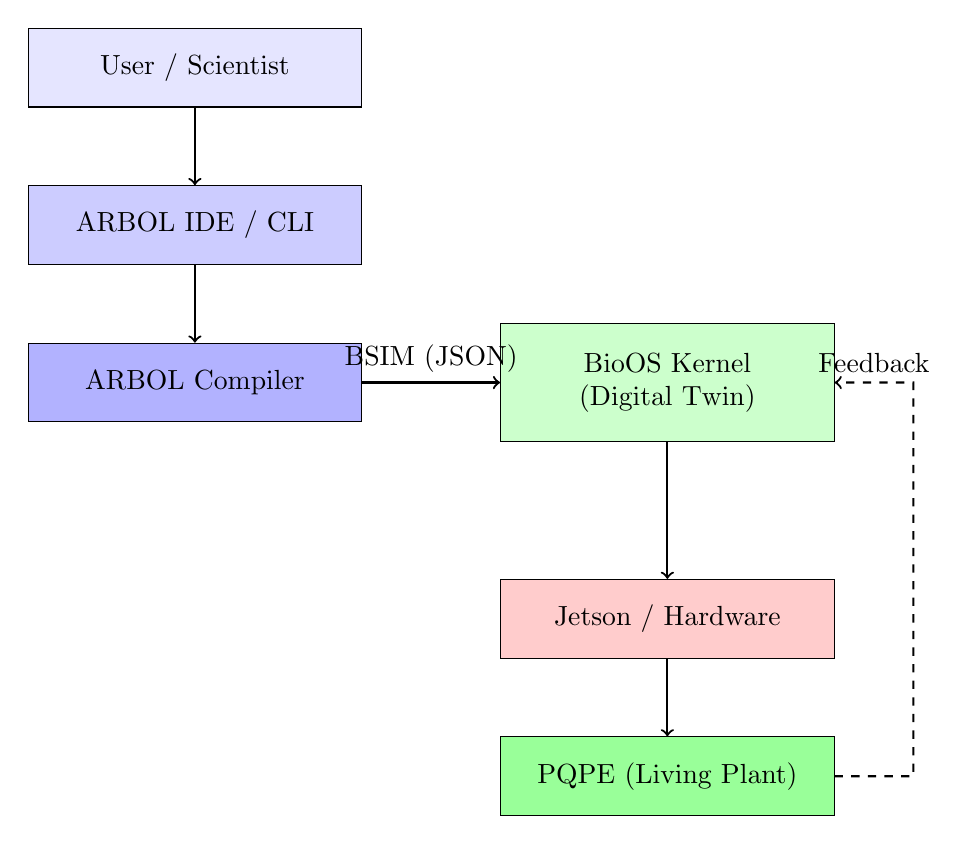
\begin{tikzpicture}[node distance=2cm, auto]
    % Nodes
    \node [rectangle, draw, fill=blue!10, text width=4cm, text centered, minimum height=1cm] (user) {User / Scientist};
    \node [rectangle, draw, fill=blue!20, text width=4cm, text centered, minimum height=1cm, below of=user] (arbol) {ARBOL IDE / CLI};
    \node [rectangle, draw, fill=blue!30, text width=4cm, text centered, minimum height=1cm, below of=arbol] (compiler) {ARBOL Compiler};
    \node [rectangle, draw, fill=green!20, text width=4cm, text centered, minimum height=1.5cm, right of=compiler, xshift=4cm] (bioos) {BioOS Kernel \\ (Digital Twin)};
    \node [rectangle, draw, fill=red!20, text width=4cm, text centered, minimum height=1cm, below of=bioos, yshift=-1cm] (hardware) {Jetson / Hardware};
    \node [rectangle, draw, fill=green!40, text width=4cm, text centered, minimum height=1cm, below of=hardware] (pqpe) {PQPE (Living Plant)};

    % Path
    \draw [->, thick] (user) -- (arbol);
    \draw [->, thick] (arbol) -- (compiler);
    \draw [->, thick] (compiler) -- node[above] {BSIM (JSON)} (bioos);
    \draw [->, thick] (bioos) -- (hardware);
    \draw [->, thick] (hardware) -- (pqpe);
    \draw [->, thick, dashed] (pqpe.east) -- ++(1,0) -- ++(0,5) -- node[above, sloped] {Feedback} (bioos.east);
\end{tikzpicture}
\caption{Conceptual flow of the HAWRA stack, from high-level ARBOL code to biological execution.}
\label{fig:global_arch}
\end{figure}

\section{Bio-Quantum Data Workflow}
The flow of information within a HAWRA node is governed by the interaction between photonic stimuli and metabolic responses.

\begin{figure}[h!]
\centering
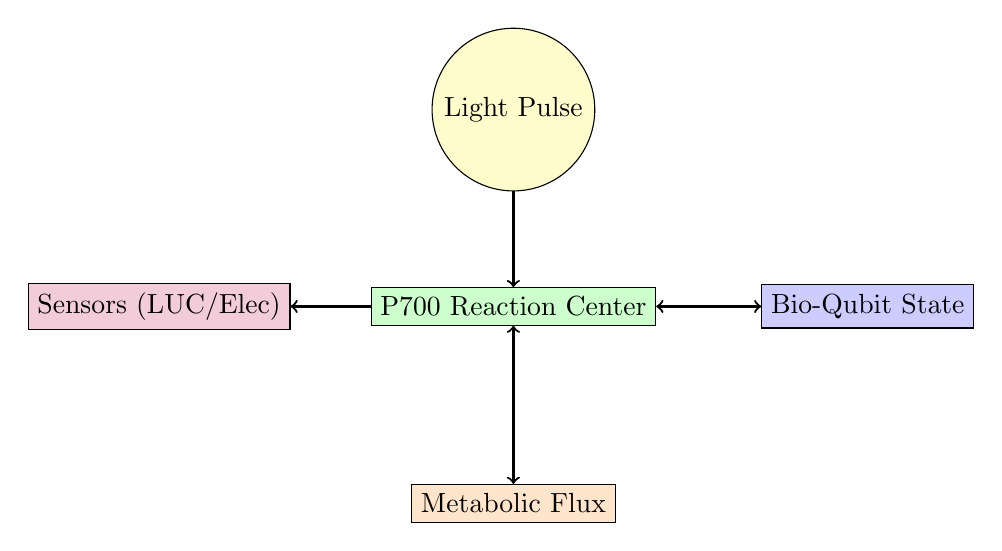
\begin{tikzpicture}[node distance=2.5cm, auto]
    % Nodes
    \node [circle, draw, fill=yellow!20] (light) {Light Pulse};
    \node [rectangle, draw, fill=green!20, below of=light] (center) {P700 Reaction Center};
    \node [rectangle, draw, fill=blue!20, right of=center, xshift=2cm] (qubit) {Bio-Qubit State};
    \node [rectangle, draw, fill=orange!20, below of=center] (metabolism) {Metabolic Flux};
    \node [rectangle, draw, fill=purple!20, left of=center, xshift=-2cm] (sensors) {Sensors (LUC/Elec)};

    % Path
    \draw [->, thick] (light) -- (center);
    \draw [<->, thick] (center) -- (qubit);
    \draw [<->, thick] (center) -- (metabolism);
    \draw [->, thick] (center) -- (sensors);
\end{tikzpicture}
\caption{Internal data and energy flow within the PQPE substrate during a quantum operation.}
\label{fig:data_workflow}
\end{figure}

\section{Execution Pipeline: Digital Twin Synchronization}
The BioOS executes every instruction in parallel on a "Digital Twin" simulator to predict metabolic stress before physical application.

\begin{figure}[h!]
\centering
\begin{tikzpicture}[node distance=1.5cm, auto]
    % Nodes
    \node [rectangle, draw, fill=gray!10] (bsim) {BSIM Instruction};
    \node [rectangle, draw, fill=blue!10, below of=bsim] (scheduler) {BioOS Scheduler};
    \node [rectangle, draw, fill=green!10, below left of=scheduler, xshift=-2cm, yshift=-1cm] (sim) {Unified Simulator};
    \node [rectangle, draw, fill=red!10, below right of=scheduler, xshift=2cm, yshift=-1cm] (phys) {Physical PQPE};
    \node [diamond, draw, fill=yellow!10, below of=scheduler, yshift=-3cm] (check) {Safety Check?};

    % Path
    \draw [->, thick] (bsim) -- (scheduler);
    \draw [->, thick] (scheduler) -| (sim);
    \draw [->, thick] (sim) |- (check);
    \draw [->, thick] (check) -| node[right, near start] {Pass} (phys);
    \draw [->, thick] (phys) -- ++(3,0) -- ++(0,5) -- (scheduler);
\end{tikzpicture}
\caption{The HAWRA execution pipeline featuring real-time Digital Twin synchronization.}
\label{fig:execution_pipeline}
\end{figure}
